\Chapter{Aufbau}
%Bild von der Versuchsanordnung einfügen
\begin{figure}[htbp]
    \centering

    \begin{subfigure}[t]{0.48\textwidth}
        \centering
        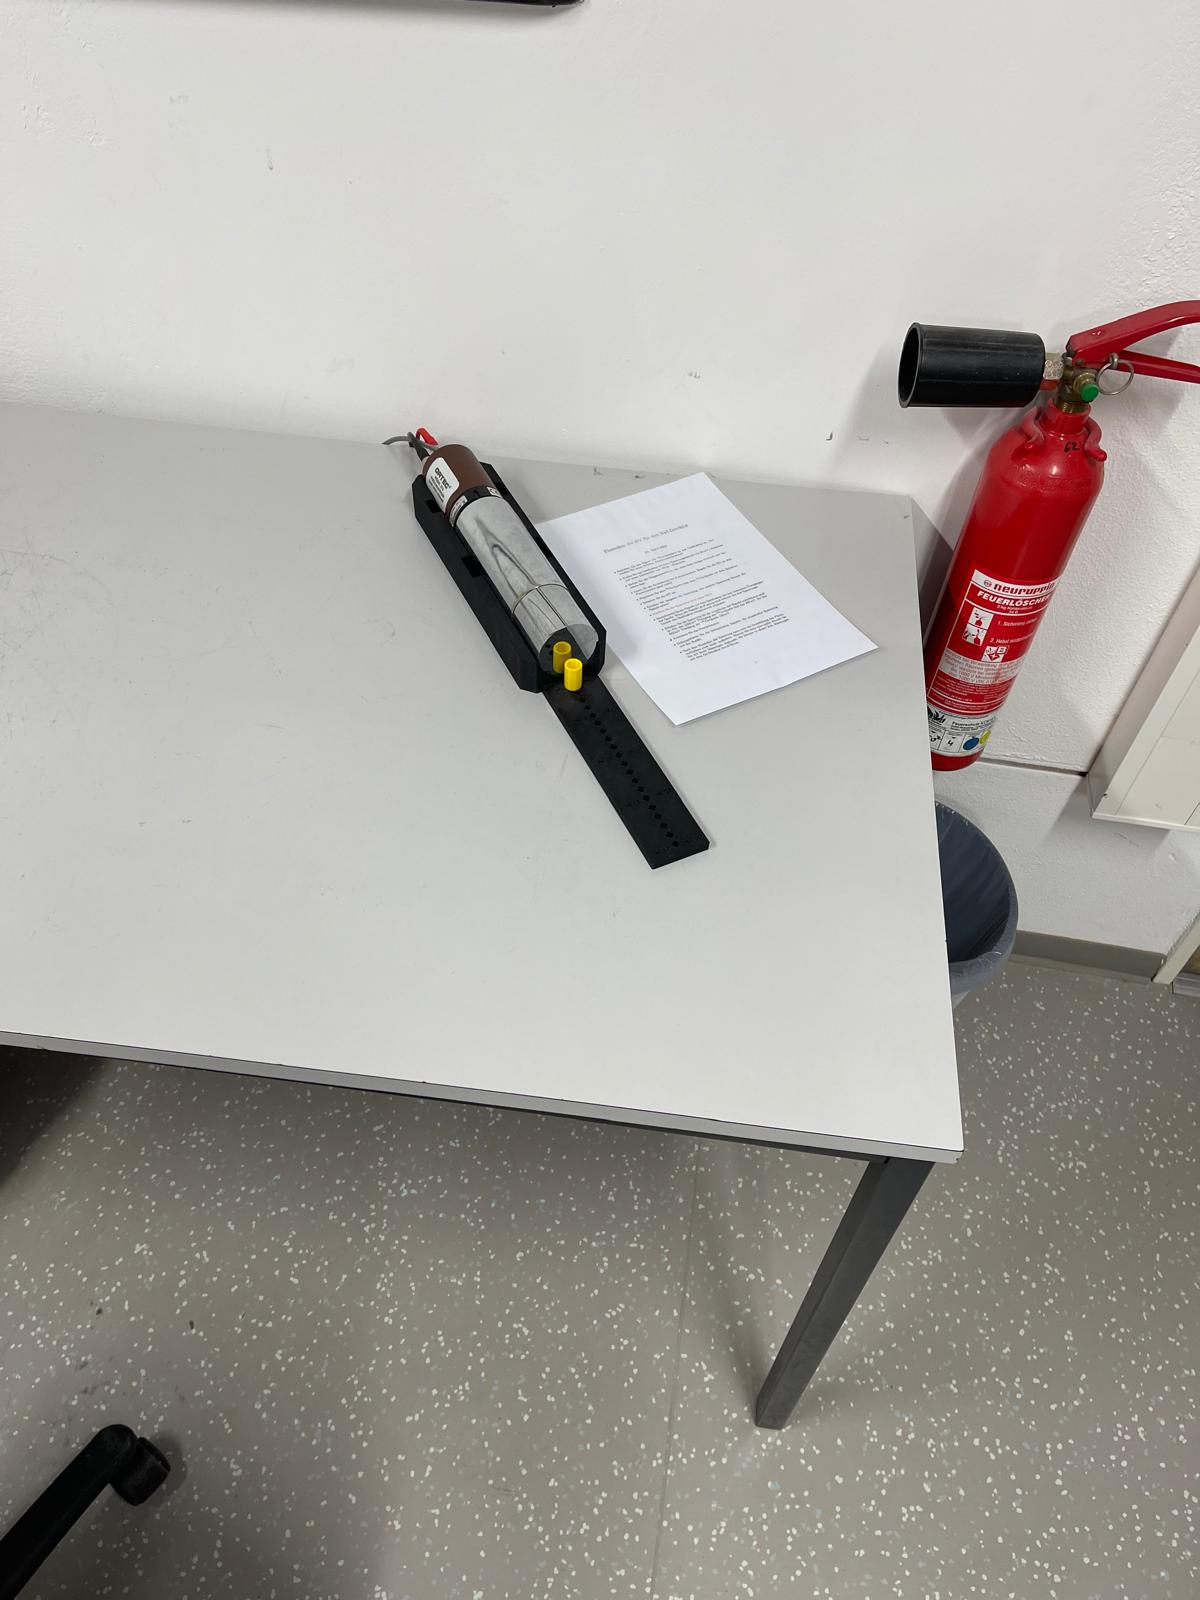
\includegraphics[width=\linewidth]{figs/NaI-detektor.jpeg}
        \caption{NaI-Szintillationsdetektor}
        \label{fig:kalib_1_1}
    \end{subfigure}
    \hfill
    \begin{subfigure}[t]{0.48\textwidth}
        \centering
        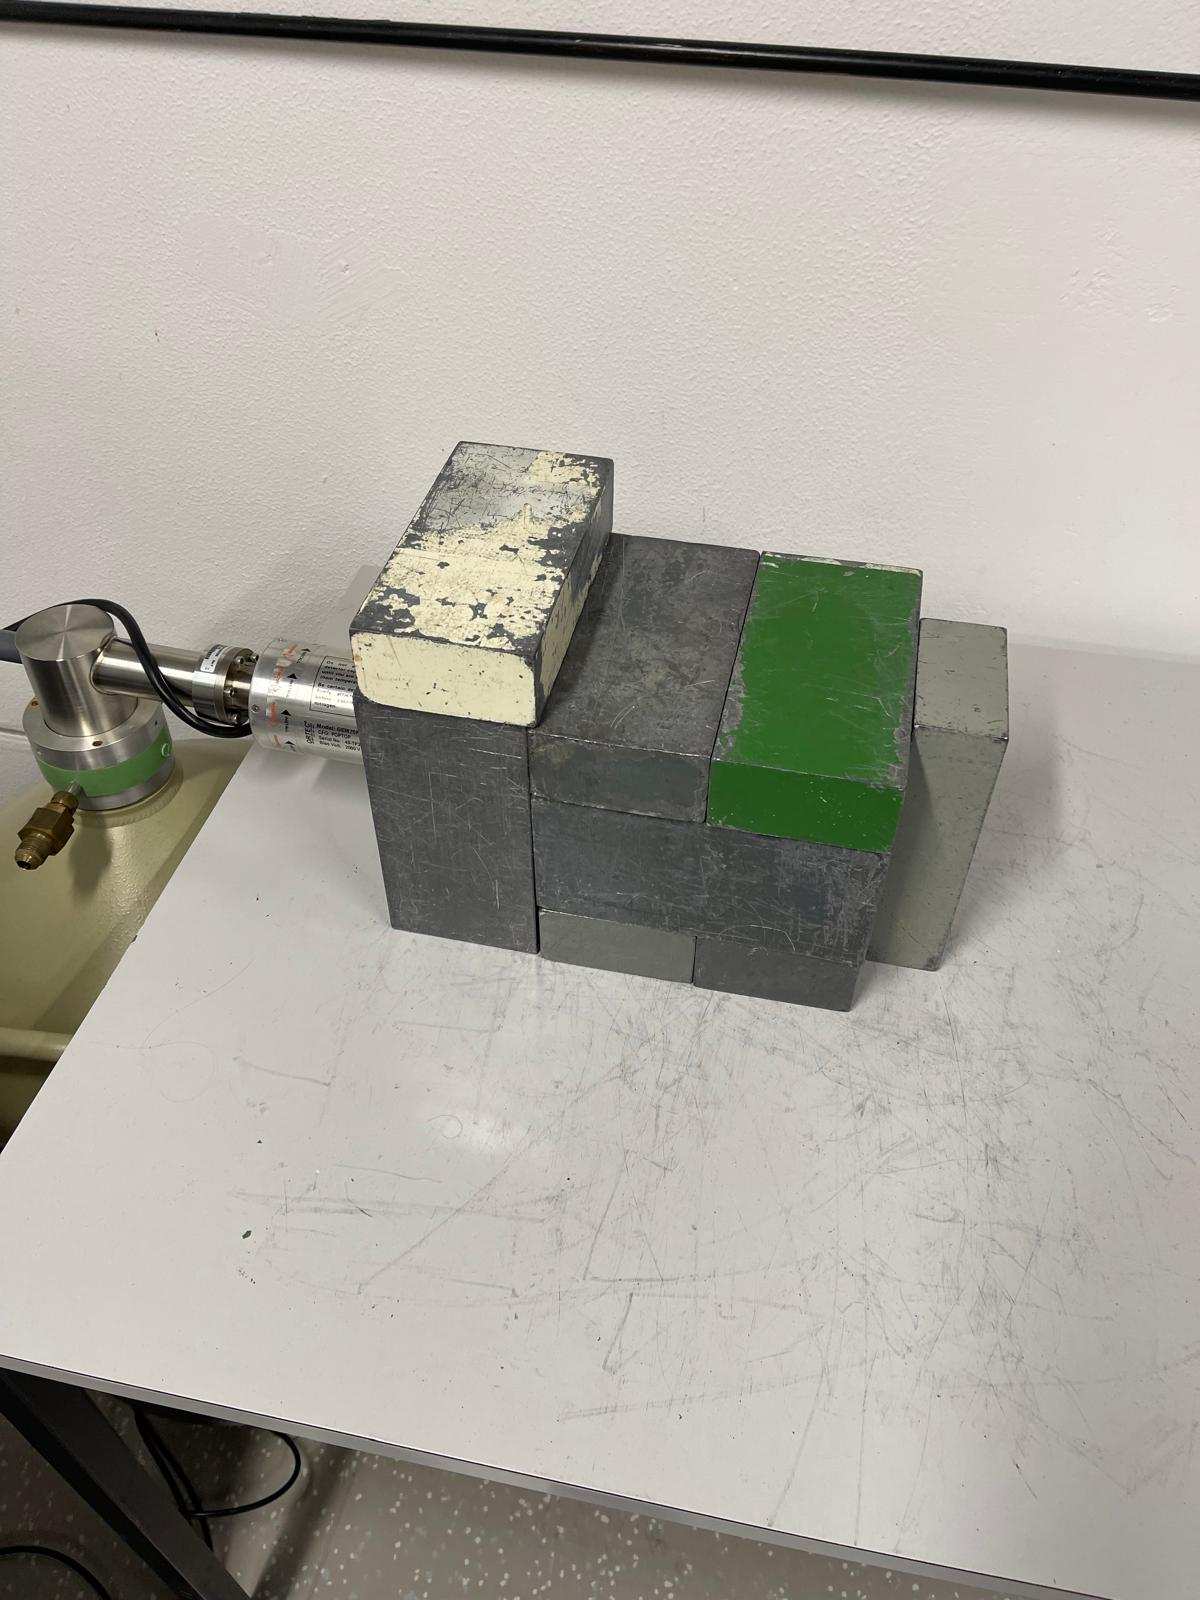
\includegraphics[width=\linewidth]{figs/HPGe_detektor.jpeg}
        \caption{HPGe-Halbleiterdetektor}
        \label{fig:kalib_1_2}
    \end{subfigure}

    \caption{Gemessenes Energie-Spektrum der $^{60}$Co-Quelle an beiden Detektoren}
    \label{fig:kalib_1}
\end{figure}
Für die Durchführung des Versuchs stehen neben den beiden Detektoren ein Vielkanalanalysator (MCA) und ein Oszilloskop zur Verfügung. Der MCA besteht aus einem Impulsverstärker, dessen Parameter mithilfe der Software MC2 Analyzer optimiert werden können.

Die Wärmequellen ($^{60}$Co, $^{137}$Cs und $^{152}$Eu) wurden in unterschiedlichen Abständen vor dem Detektor auf einem verstellbaren Gitter positioniert. Der Abstand zwischen Probenmitte und Detektorspitze wurde mithilfe einer Skala eingestellt, um die Genauigkeit der geometrischen Messungen zu gewährleisten.

Der Durchmesser des aktiven Kristalls betrug 50,8 mm für den HPGe-Detektor und 55,7 mm für den NaI(Tl)-Detektor. Abbildung ??? zeigt die beiden Detektoren während des Experiments.
